\documentclass[a4paper,12pt]{article}
\usepackage{float}
\usepackage{hyperref}
\usepackage{graphicx}

\title{Final report}
\author{The Waypointers}

\begin{document}

%%%%%%%%%%%%%%%%%%%%%%%%%%%%%%%%%%%%%%%%%
% University Assignment Title Page
% LaTeX Template
%
% This template has been downloaded from:
% http://www.LaTeXTemplates.com
%
% Original author:
% WikiBooks (http://en.wikibooks.org/wiki/LaTeX/Title_Creation)
%
% License:
% CC BY-NC-SA 3.0 (http://creativecommons.org/licenses/by-nc-sa/3.0/)i

\begin{titlepage}

\newcommand{\HRule}{\rule{\linewidth}{0.5mm}} % Defines a new command for the horizontal lines, change thickness here

\center % Center everything on the page

%----------------------------------------------------------------------------------------
%	HEADING SECTIONS
%----------------------------------------------------------------------------------------

\textsc{\LARGE King's College London}\\[1.5cm] % Name of your university/college
\textsc{\Large 7CCSMGPR Group Project}\\[0.5cm] % Major heading such as course name
%\textsc{\large Minor Heading}\\[0.5cm] % Minor heading such as course title

%----------------------------------------------------------------------------------------
%	TITLE SECTION
%----------------------------------------------------------------------------------------

\HRule \\[0.4cm]
{ \huge \bfseries Final project report}\\[0.4cm] % Title of your document
\HRule \\[1.5cm]

%----------------------------------------------------------------------------------------
%	AUTHOR SECTION
%----------------------------------------------------------------------------------------
\begin{flushleft}
{\Large \emph{Team:}\\
\textsc{The Waypointers}\\}
Haipei Liu\\
Karlo Santini\\
Michal Szewczak\\
Mengzhu Wang\\
Minghao Zhu\\[3cm]
\end{flushleft}
%----------------------------------------------------------------------------------------
%	DATE SECTION
%----------------------------------------------------------------------------------------

{\large \today}\\[3cm] % Date, change the \today to a set date if you want to be precise

%----------------------------------------------------------------------------------------
%	LOGO SECTION
%----------------------------------------------------------------------------------------

%\includegraphics{Logo}\\[1cm] % Include a department/university logo - this will require the graphicx package

%----------------------------------------------------------------------------------------

\vfill % Fill the rest of the page with whitespace

\end{titlepage}

%%%%%%%%%%%%%%%%%%%%%%%%%%%%%%%%%%%%%%%%%%

\tableofcontents

\section{Introduction}
The Traffic Simulation System aims to provide users to create a traffic map as they wish. In general, there are three parts in the system: MapPanel, ControlPanel and StatisticsPanel. MapPanel is to show how the traffic map is built while ControlPanel is for users to decide what their traffic map looks like and how do vehicles behave. StatisticsPanel reveals the average speed of different types of vehicles.

Users can control the whole system by clicking start, pause and clear buttons, changing time step, vehicle speed and states, and even using 'debug' to follow every car track and the location of junctions. Specifically, there are four types of vehicle in the system, namely caution cars, normal cars, reckless cars and ambulance. Each type of them have different behaviors, such as speed. The system allows users to decide how many cars run on the road. Users can also choose whether there are traffic lights on junctions or not. They can also change traffic lights' time interval.

\section{Review of related work}

\section{Requirements}

\section{Design}

\section{Implementation}

\subsection{GUI part}

Basically, GUI is to display performance of the whole system, showing the results of how the system runs. In GUI, we draw traffic road on class MapPanel. The MapPanel mainly consist of five parts: to paint road, vehicle, traffic lights, labels and to get statistical data.

\subsubsection{compute$\_$xy( )}
When drawing road, we get the junctions and roads from background. One thing we have to deal with is to compute the coordinate of each junction and road, then draw them on the MapPanel. We assume that the first junction we get from our background is on the top left of the map. So we make the coordinate as $(x,y)=(road_length, road_length)$. Afterwards, based on the location of the first junction, we compute the rest roads and junctions until finishing the whole map. On the contrary, if the first junction we get is not located on the top left, then we move the junction to its correct location. As long as we complete the road map, achieving coordinate of each junction, we can easily compute the relative coordinates of vehicle and traffic lights. Finally, we draw the whole traffic map.

\subsubsection{drawVehicleInJunction( )}
Considering vehicles turning on junctions, we first divide turning situation into the following eight parts, where $\alpha$ represents its turning angle. Then using Java function, AffineTransform(), to rotate the vehicle towards its right way.
\begin{center}
	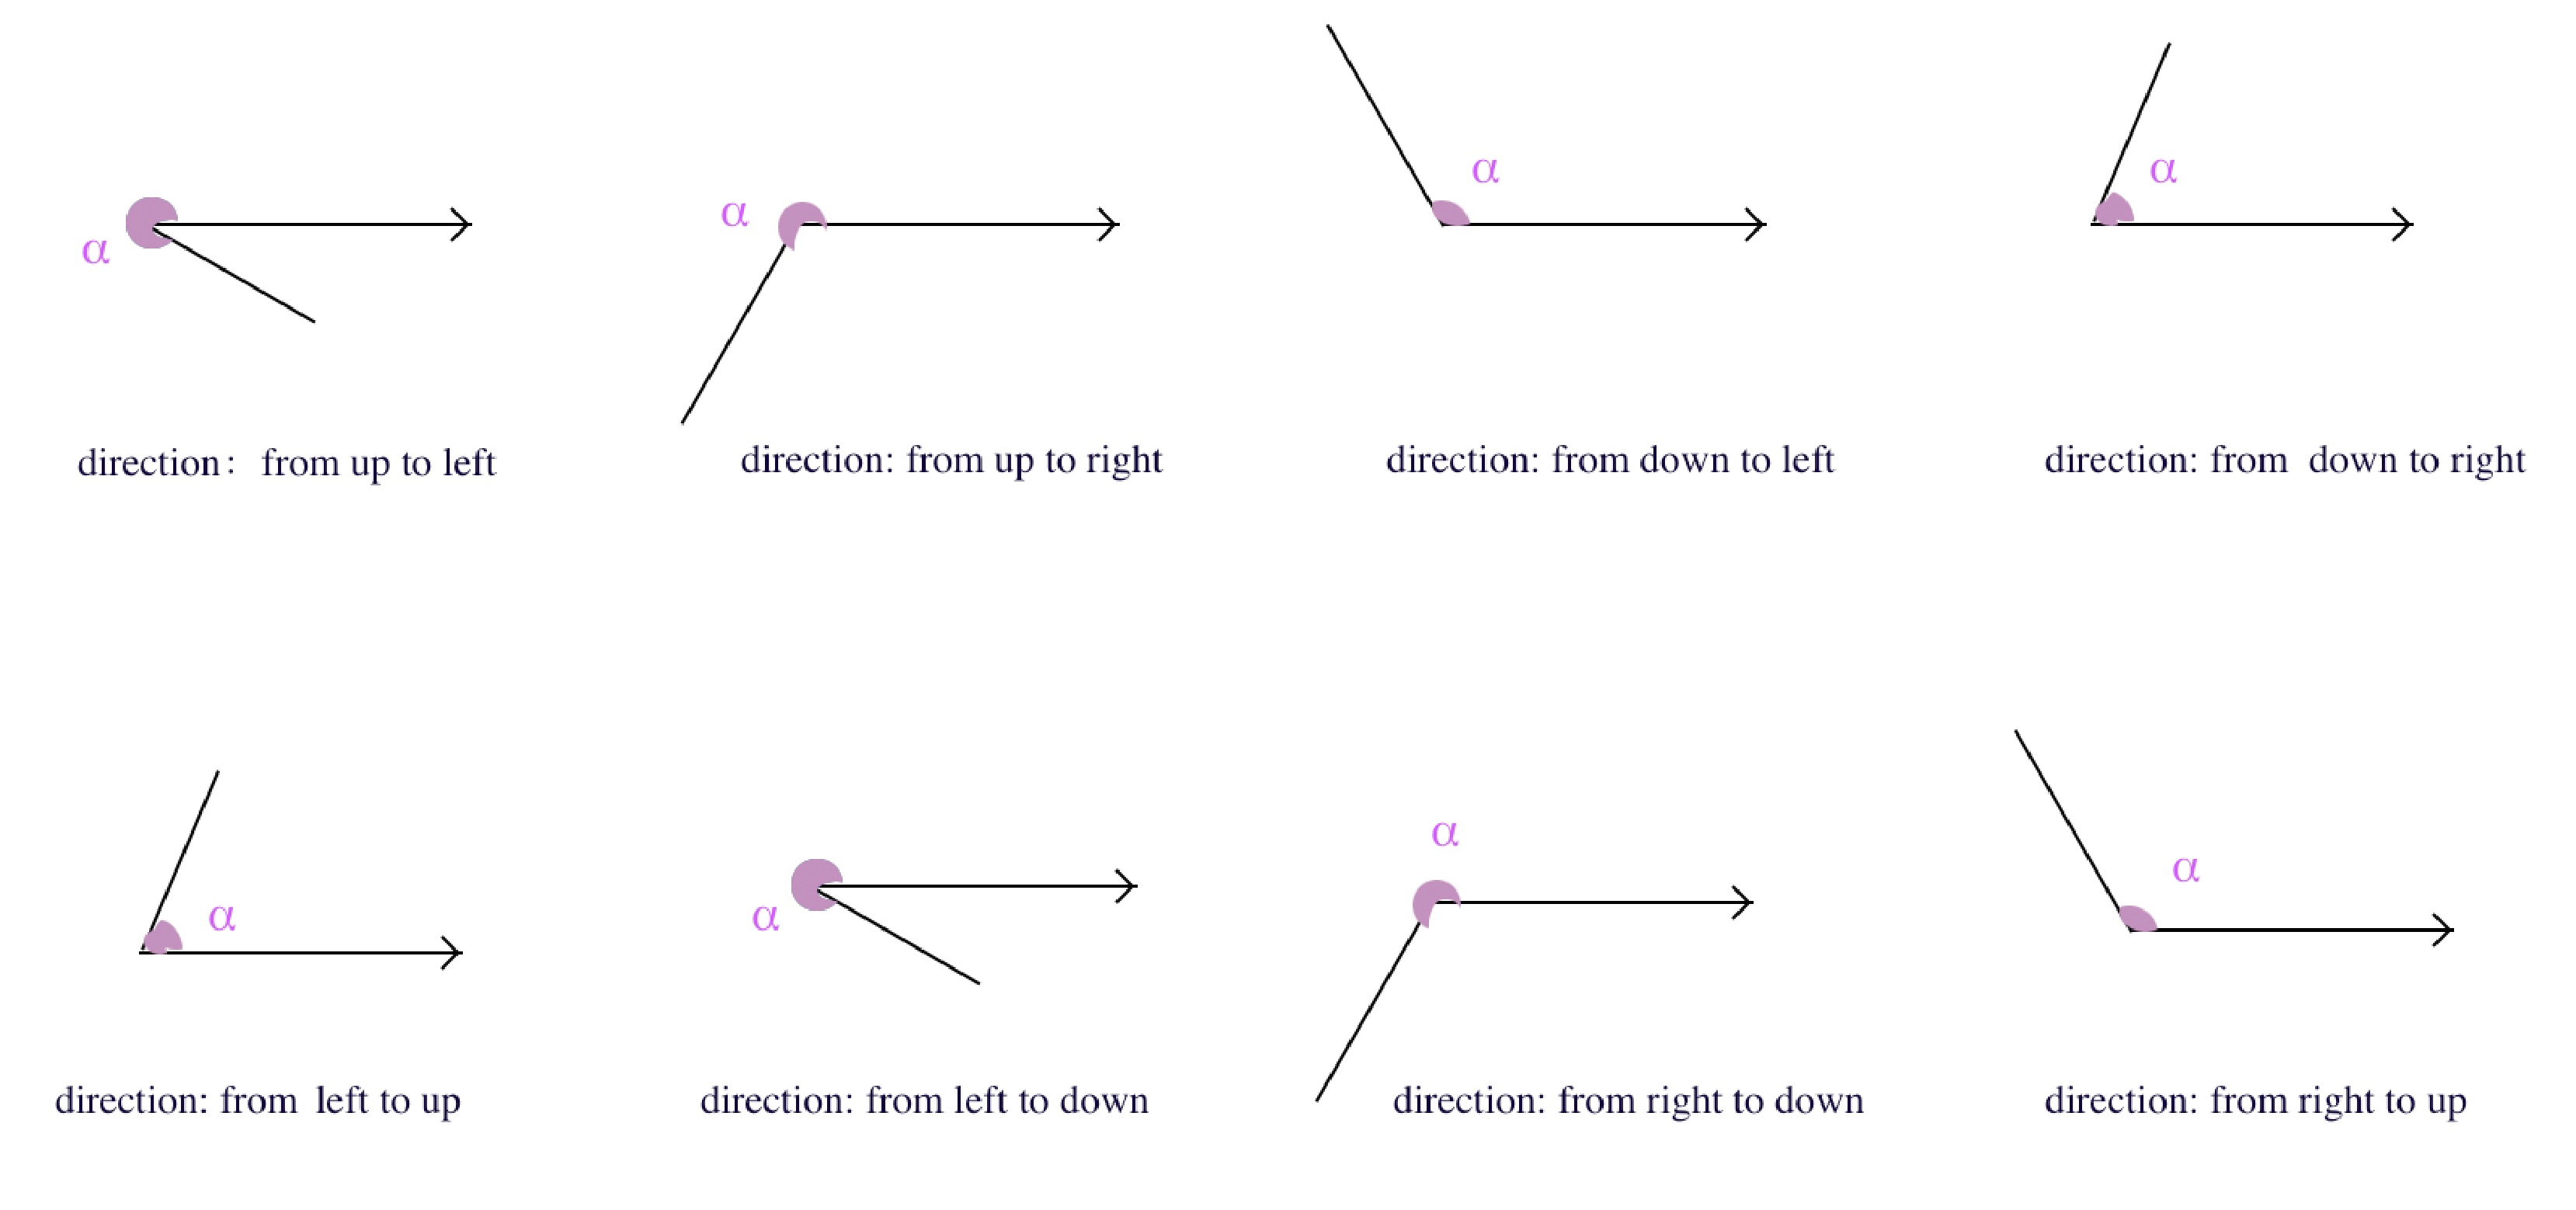
\includegraphics[width=14cm]{GUI_p1.eps}
\end{center}

\subsubsection{RecordStatistics( )}
Our system will collect the travel distance of every car and then compute their average speed for further analysis, showing on StatisticsPanel. We create a list for the whole system and list information for cars, running time and running distance. The pseudo-code shows as below:
\begin{center}
	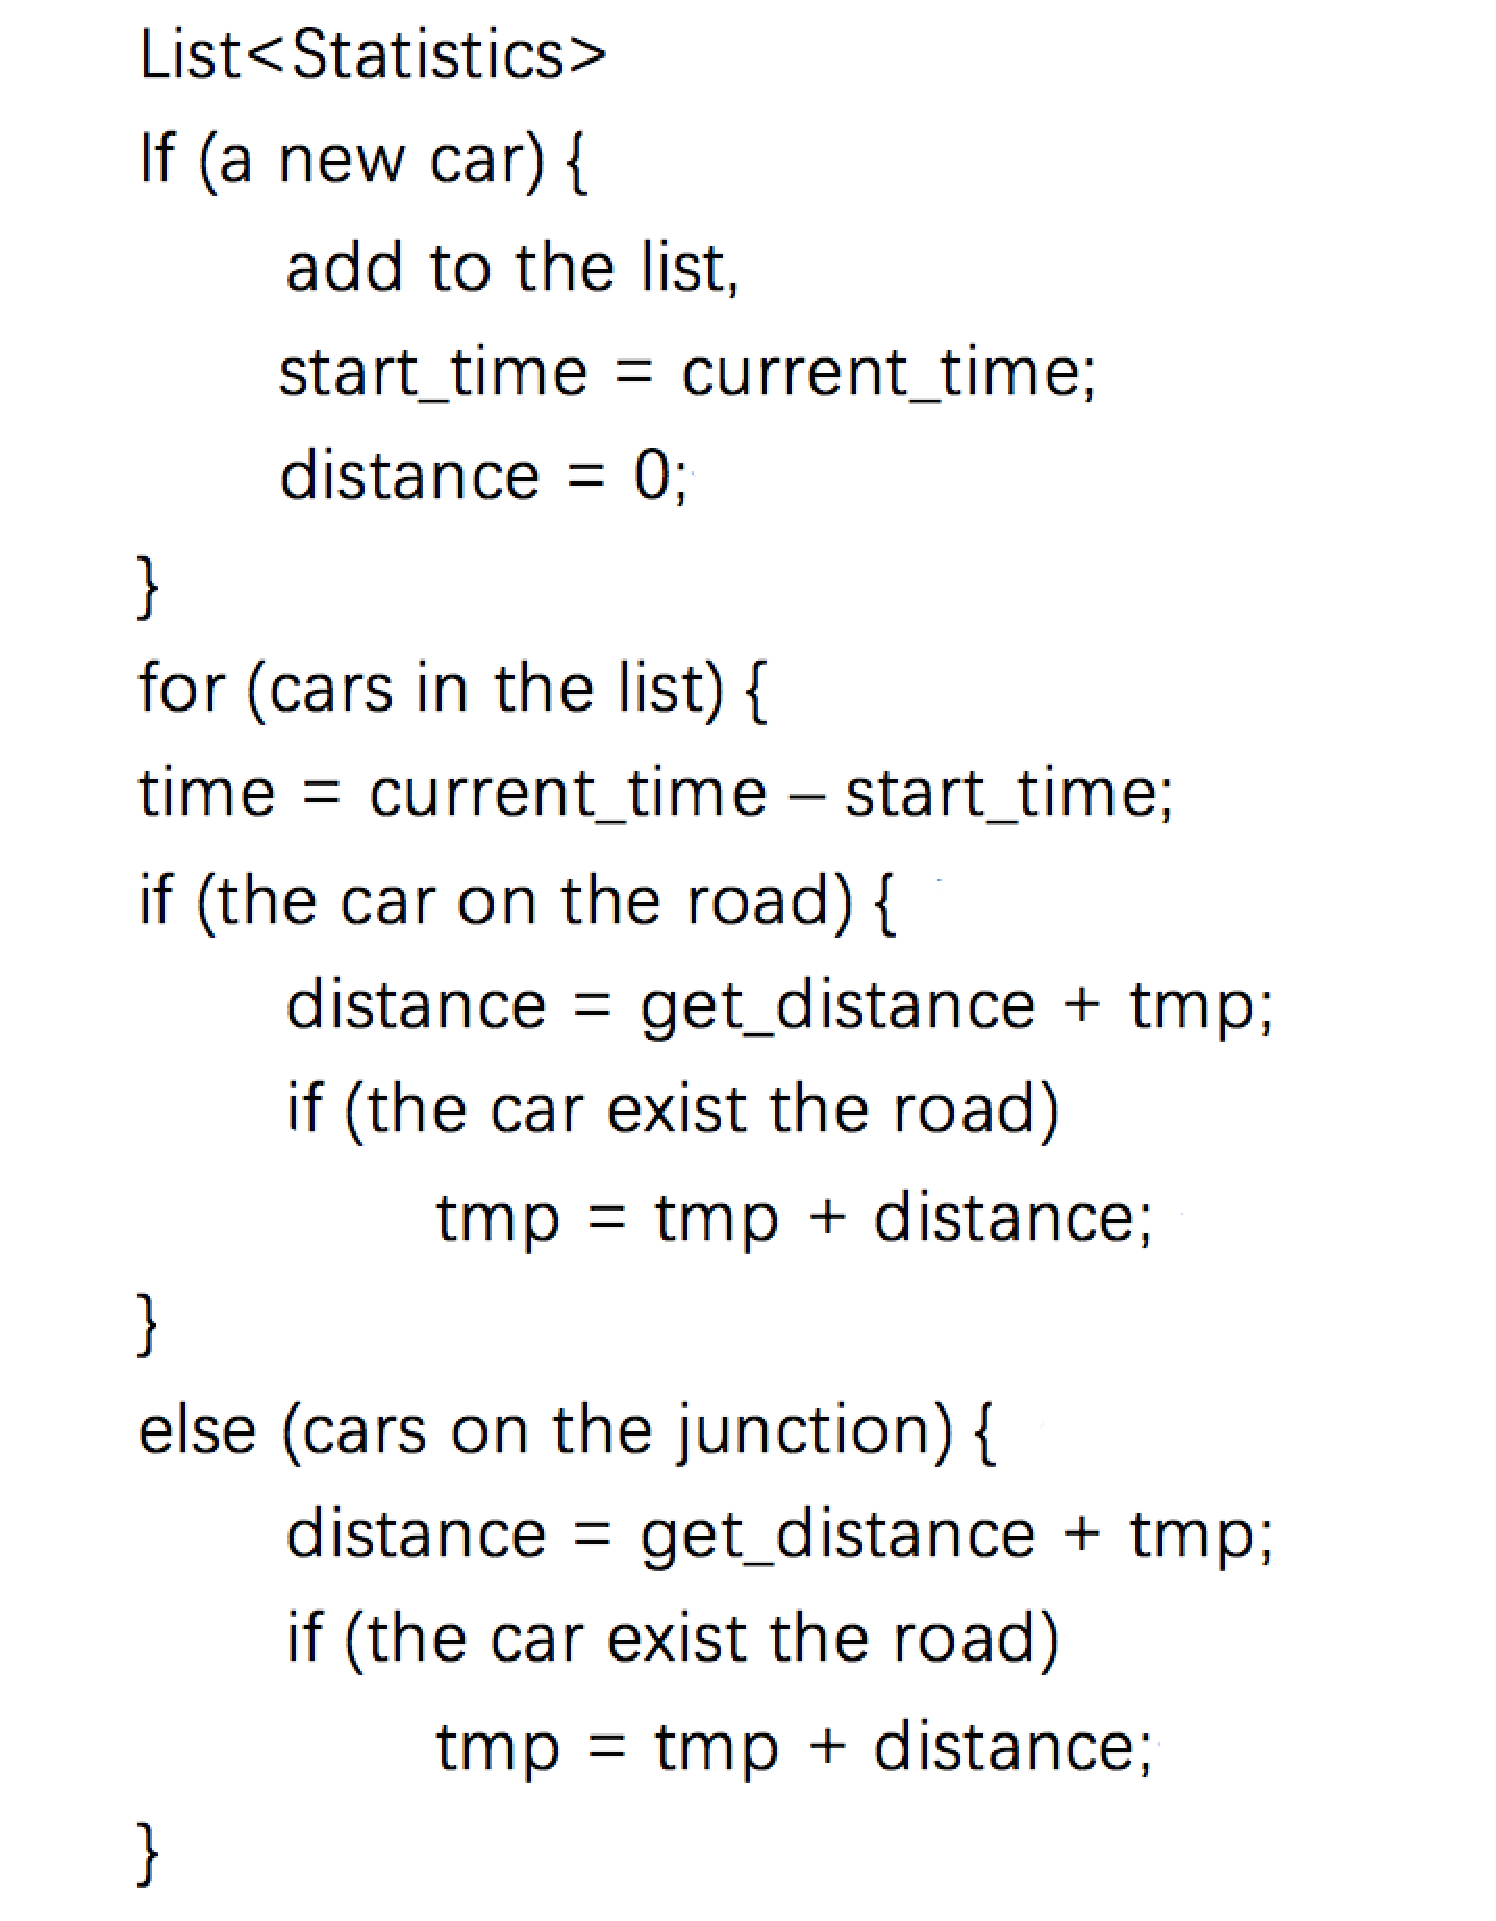
\includegraphics[width=6cm] {GUI_p2.eps}
\end{center}

\section{Teamwork}

\subsection{Tools and libraries used}

\subsubsection*{Tools and applications}

\begin{itemize}
	\item Git\footnote{\url{https://git-scm.com/}} - version control
	\item GitHub\footnote{\url{https://github.com/}} - Git repository management, task assignment, teamwork
	\item \LaTeX\footnote{\url{https://www.latex-project.org/}} - typesetting system, for creating documentation
	\item Gliffy\footnote{\url{https://www.gliffy.com/}} - a Chrome app for creating diagrams
	\item Apache Maven\footnote{\url{https://maven.apache.org/}} - a build tool for building the project easily and for dependency management
	\item Travis CI\footnote{\url{https://travis-ci.org/}} - a continuous integration tool that integrates into GitHub and builds every commit pushed to the repository (in our case - using Maven), also checking if the tests pass
	\item IntelliJ IDEA\footnote{\url{https://www.jetbrains.com/idea/}} - a cross-platform IDE for development in Java (and more). To minimize potential hassles with different development environments, we all agreed on using the same IDE.
\end{itemize}


A significant fact to note that is our team used all the major operating systems (Windows, OS X, Linux), so we focused on choosing cross-platform tools. The only troubles that arised from that were minor layout differences in the Swing GUI of our system.

\subsubsection*{Libraries}

\begin{itemize}
	\item JDK 1.8\footnote{\url{http://www.oracle.com/technetwork/java/javase/downloads/index.html}} - We had several reasons for choosing Java: \begin{itemize}
		\item Familiarity of team members with it
		\item Available on all platforms
		\item Good capabilities of cross-platform GUI
		\item Strong typing allowing for easier maintaining of code integrity
	\end{itemize}
	We chose version 8 because it introduces many much-needed improvements for the language like lambda functions or the Stream API.
	\item JUnit 4.12\footnote{\url{http://junit.org/junit4/}} - The ``de facto'' unit testing library for Java. Good integration with IntelliJ IDEA and Maven.
	\item FEST-Assert 2.0M5\footnote{\url{https://github.com/alexruiz/fest-assert-2.x}} - A library to make assertions in unit tests more readable and easier to compose.
	\item JGraphT 0.7.3 \footnote{\url{http://jgrapht.org/}} - A graph library to take advantage of graph representation of the road network, mainly pathfinding for vehicles.
	\item XStream 1.2.2 \footnote{\url{http://x-stream.github.io/}} - An XML serialization library to bring reading and writing XML road maps to life.
\end{itemize}



\section{Evaluation}

\section{Peer assessment}

\end{document}
